\documentclass[11pt]{ligovirgodcc}

\usepackage{graphicx}
\usepackage{hyperref}
\usepackage{amssymb}
\usepackage{amsmath}
\usepackage{longtable}
\usepackage{rotating}
\usepackage{color}
\usepackage{epsfig}
\usepackage{epsf}
\usepackage{fancyhdr}
\usepackage{ifthen}
\usepackage{psfrag}
\usepackage{comment}
\usepackage{float}
\usepackage{listings}
\begin{document}

%\pdfgraphics
\pagestyle{fancy}
\chead[LALSimulation Chirplets]
      {LALSimulation Chirplets}
\rhead[]{}
\lhead[]{}
%
\title{Chirplets In LALSimulation}

\ligodocdraft{\hfill}
\ligodoc{LIGO-XXXXXXXX-v1}{X}

\author{J.~Clark}
%
\date{\today}

%
\maketitle

\tableofcontents
\newpage
\lstset{language=Python}
\section{Introduction}
This document describes a proposed chirplet waveform for use in {\tt
LALSimulation} and integration into {\tt LALInference}.  The proposed waveform
is described in~\cite{2010CQGra..27s4017C}.  We'll just copy and build on that
description.

\section{Definition of Chirplets}
\subsection{Time Domain}
Define the time-domain chirplet as:
\begin{equation}
\psi(t) \equiv A \exp\left\{-\frac{(2\pi
f_0)^2}{Q^2}(t-t_0)^2\right\} \exp \left\{ 2\pi i [ f_0 +
\mathcal{D}/2(t-t_0)^2 ] + \phi_0 \right\},
\end{equation}
%
where $t_0$ and $f_0$ are the center time and frequency, respectively and
$\phi_0$ is an arbitrary initial phase.  Following~\cite{2010CQGra..27s4017C},
quality factor $Q$ is,
\begin{equation}
Q = 2\sqrt{\pi} f_0 \tau,
\end{equation}
%
where $\tau$ is the chirplet duration,
\begin{equation}
\tau \equiv 2\sqrt{\pi} \int_T (t-t_0)^2 |\psi(t)|~\mathrm{d}t.
\end{equation}
%
The amplitude $A$ is a normalisation term,
\begin{equation}
A = \left(\frac{8\pi f_0^2}{Q^2}\right)^{1/4},
\end{equation}
%
which ensures $\int_T |\psi(t)|^2~\mathrm{d} t = 1$.  The quantity $\mathcal{D}$
is the \emph{chirp rate}, which controls the frequency evolution so that the
instantaneous frequency evolves linearly as $f(t) = f_0 + \mathcal{D}(t-t_0)$.
The waveform reduces to the familiar sine-Gaussian when $\mathcal{D}=0$.  It's
worth emphasising here that these are linear chirps.  It is easy to imagine
reparameterising to allow for (e.g.,) power-law or polynomial frequency
evolution\footnote{see e.g.,
\url{http://docs.scipy.org/doc/scipy-0.14.0/reference/generated/scipy.signal.chirp.html}}.

With the basis waveform $\psi(t)$ thus defined, the polarisations for a
time-domain linear chirplet in {\tt LALSimulation} are,
\begin{eqnarray}
h_+(t|h_{\mathrm{rss}},\alpha,f_0,t_0,\phi_0,Q,\mathcal{D}) & = &
\Re\left[h_{\mathrm{rss}} \cos (\alpha)
\psi(t|f_0,t_0,\phi_0,Q,\mathcal{D})\right] \\
h_{\times}(t|h_{\mathrm{rss}},\alpha,f_0,t_0,\phi_0,Q,\mathcal{D}) & = & \Im
\left[h_{\mathrm{rss}} \sin (\alpha) \psi(t|f_0,t_0,\phi_0,Q,\mathcal{D})
\right]
\end{eqnarray}
%
where $\alpha$ is a polarisation angle to control the ellipticity of the
waveform and $h_{\mathrm{rss}}$ is the root-sum-squared amplitude,
\begin{equation}
\label{eq:hrss}
h_{\mathrm{rss}} = \sqrt{\int_T |h_+(t)|^2 + |h_{\times}(t)|^2~\mathrm{d}t}.
\end{equation}
%
\subsection{Frequency Domain}
Following~\cite{2010CQGra..27s4017C}, the frequency domain chirplet is, 
\begin{equation}
\tilde{\psi}(f) = \mathcal{A} \exp \left[ - \frac{\tilde{Q}^2}{4}
\left(\frac{f-f_0}{f}\right)^2 + i\phi_0\right]
\end{equation}
%
where the amplitude normalisation $\mathcal{A}$ is,
\begin{equation}
{\mathcal A} = \left[ \frac{\tilde{Q}^4}{Q^2}\frac{1}{2\pi f_0^2} \right]^{1/4},
\end{equation}
%
and $\tilde{Q}$ is the complex quality factor which carries the chirp rate
$\tilde{D}$,
\begin{equation}
\tilde{Q} = Q\frac{\sqrt{z}}{|z|},
\end{equation}
%
and $z = 1 + i\mathcal{D} \tau^2$.

Then, as before, we have the frequency domain polarisations:
\begin{eqnarray}
\tilde{h}_+(f|h_{\mathrm{rss}},\alpha,f_0,\phi_0,Q,\mathcal{D}) & = &
h_{\mathrm{rss}} \cos (\alpha)
\tilde{\psi}(f|h_{\mathrm{rss}},\alpha,f_0,\phi_0,Q,\mathcal{D}) \\
\tilde{h}_{\times}(f|h_{\mathrm{rss}},\alpha,f_0,\phi_0,Q,\mathcal{D}) & = &
h_{\mathrm{rss}} \sin (\alpha)
\tilde{\psi}(f|h_{\mathrm{rss}},\alpha,f_0,\phi_0+\pi/2,Q,\mathcal{D}) 
\end{eqnarray}

\section{Examples}
Figures~\ref{fig:linpol} and~\ref{fig:circpol} show linearly- and
circularly-polarised waveforms, respectively,  generated in the time-domain with
the following call in python:% (see appendix~\ref{sec:waveform_examples} for a
%full demonstration):
\begin{lstlisting}
hp, hc = lalsim.SimBurstChirplet(Q, centre_frequency, 
    chirp_rate, hrss, alpha, phi0, delta_t)
\end{lstlisting}
%
The right panels of the figures also show the PSDs.  The epochs are computed
such that the middle sample of the waveform is $t=0$, as per the sine-Gaussian
convention.  We also confirm that the root-sum-squared strain (see
equation~\ref{eq:hrss}) is unity as requested.  This is computed using:
\begin{lstlisting}
hrss=lalsim.MeasureHrss(hp,hc).
\end{lstlisting}
%
Finally, figure~\ref{fig:fdomlinpol} shows the analytic Fourier domain waveform
returned by,
\begin{lstlisting}
hp, hc = lalsim.SimBurstChirpletF(Q, centre_frequency, 
    chirp_rate, hrss, alpha, phi0, delta_f, delta_t),
\end{lstlisting}
as well as the FFT of the time-domain waveform from {\tt SimBurstChirplet()}.
We plot the real parts of the complex Fourier spectra in the left panel and the
imaginary parts in the right panel.  We confirm that the F-domain analytic waveform
does indeed match the FFT of the T-domain waveform (ignoring the high-frequency
phase-shift oscillations in the numerical waveform).


\begin{figure}
\centering
\scalebox{0.7}{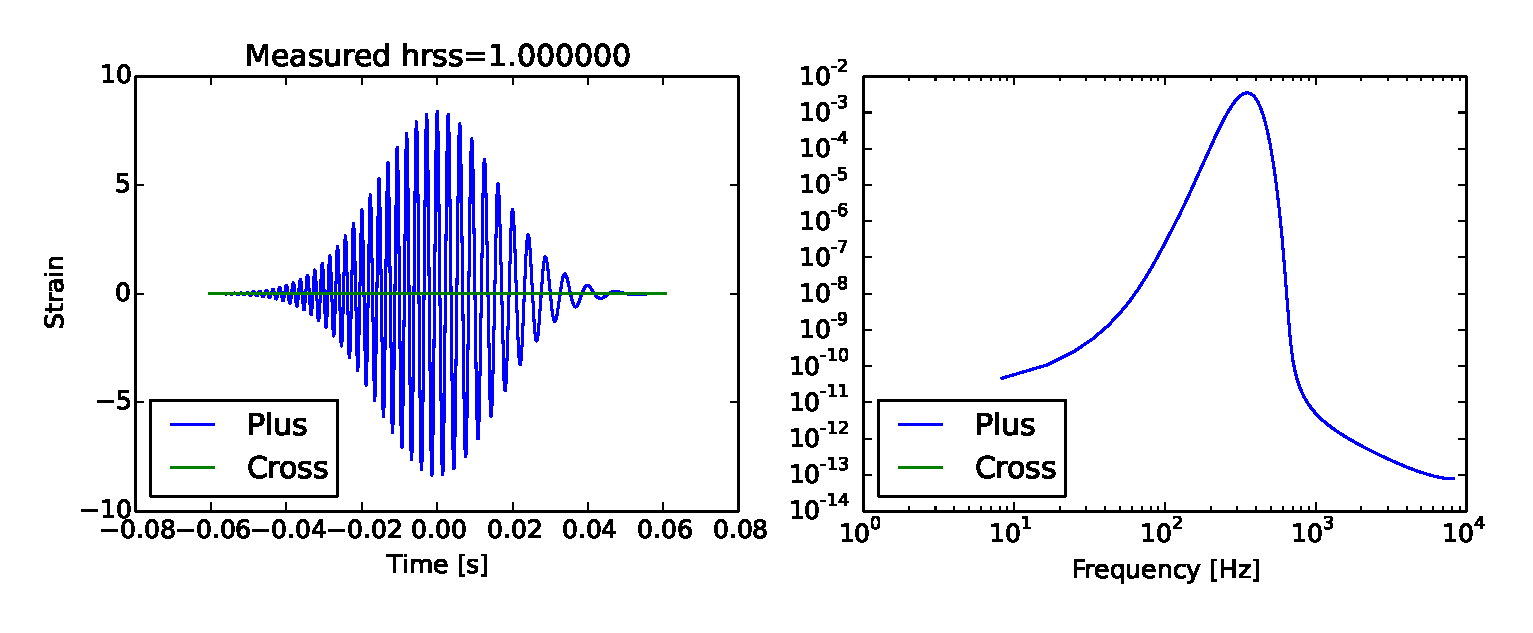
\includegraphics{LinearPol.eps}}
\caption{Linearly polarised chirplet with $h_{\mathrm{rss}}=1$, $\alpha=0$,
$Q=50$, $f_0=350$\,Hz, $\mathcal{D}=-5000$\,Hz\,s$^{-1}$.\label{fig:linpol}}
\end{figure}

\begin{figure}
\centering
\scalebox{0.7}{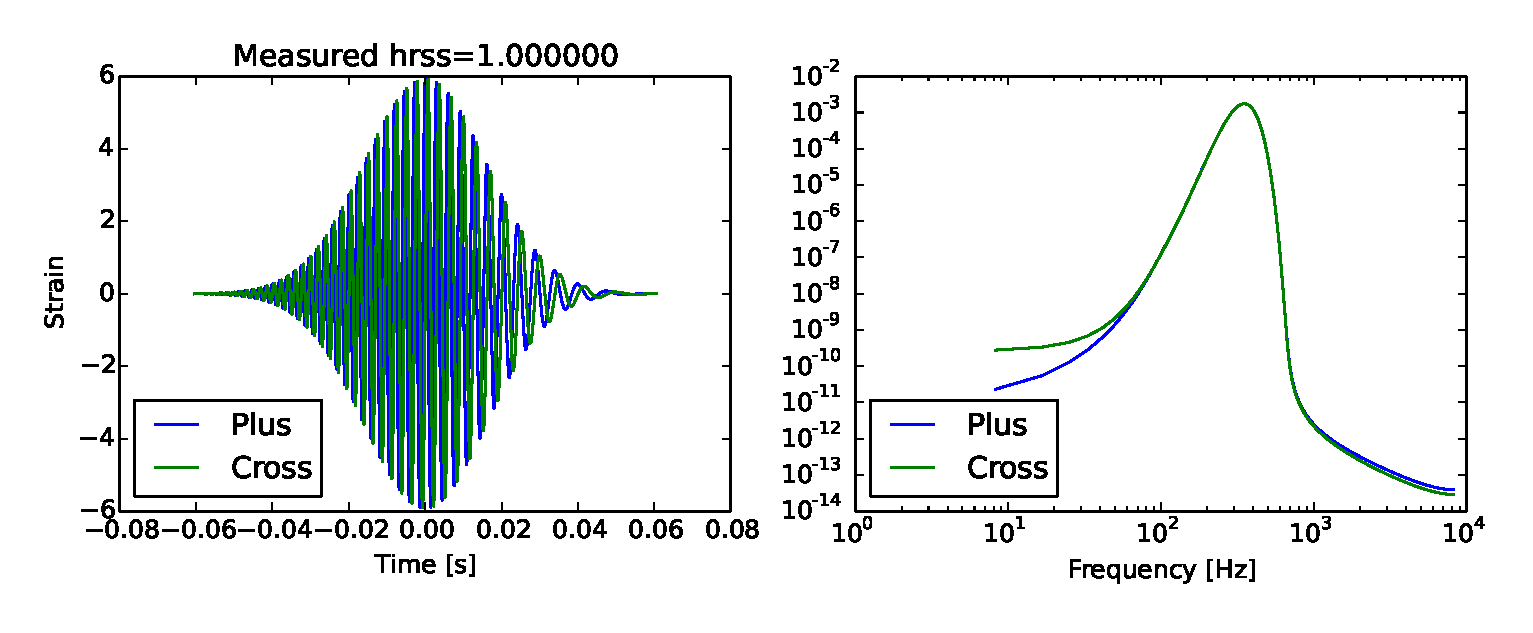
\includegraphics{CircPol.eps}}
\caption{Circularly polarised chirplet with $h_{\mathrm{rss}}=1$, $\alpha=\pi/4$,
$Q=50$, $f_0=350$\,Hz, $\mathcal{D}=-5000$\,Hz\,s$^{-1}$.\label{fig:circpol}}
\end{figure}

\begin{figure}
\centering
\scalebox{0.7}{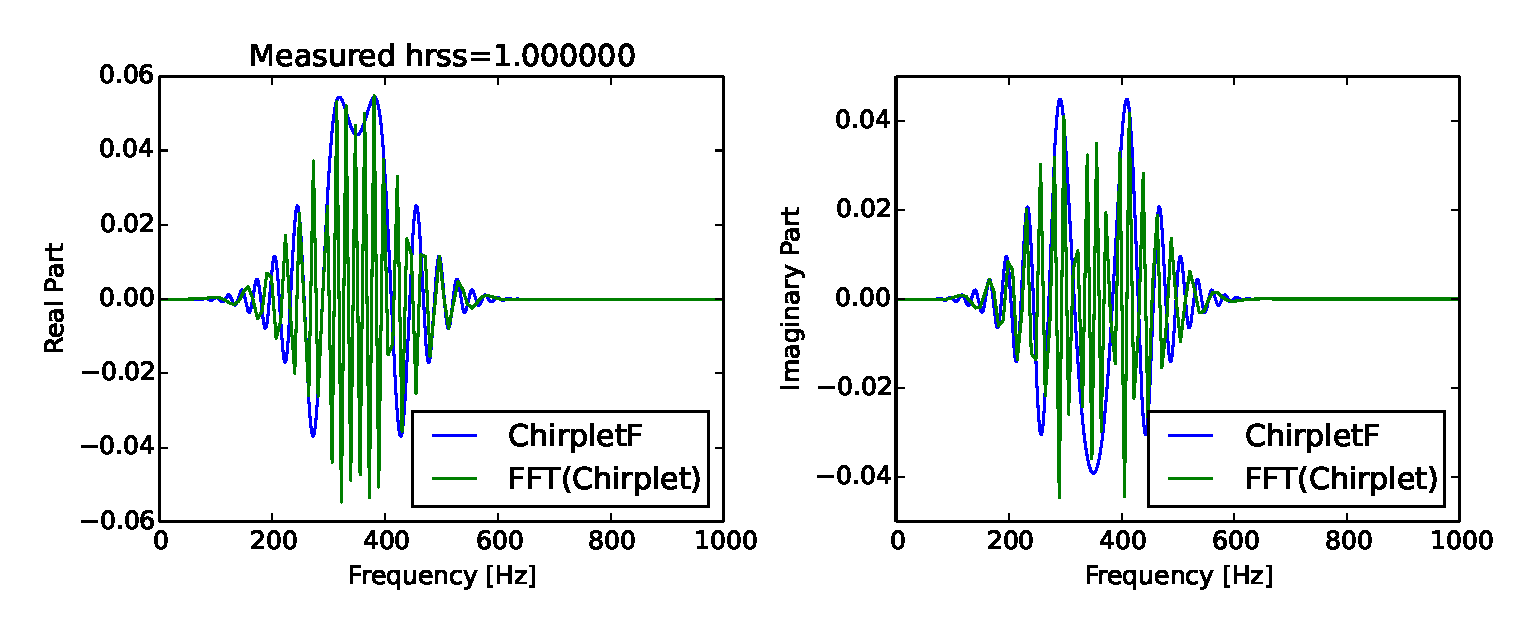
\includegraphics{FdomainLin.eps}}
\caption{Plus-polarised chirplet with $h_{\mathrm{rss}}=1$, $\alpha=\pi/4$,
$Q=50$, $f_0=350$\,Hz, $\mathcal{D}=-5000$\,Hz\,s$^{-1}$.\label{fig:fdomlinpol}.
 Left panel shows the real part of the Fourier transform, right panel shows the
 imaginary part of the Fourier transform; blue trace is the analytic Fourier
 transform, using {\tt SimBurstChirpletF()}, green trace is the FFT of the
 time-domain chirplet {\tt SimBurstChirplet()}.}
\end{figure}

%\appendix
%\section{Waveform Example Code}
%\label{sec:waveform_examples}
%\lstinputlisting[language=Python]{chirplet_demo.py}

\bibliographystyle{plain}
\bibliography{chirplets}

\end{document}

